\documentclass[a4paper,11pt,landscape,exos]{nsi} % COMPILE WITH DRAFT
\usepackage{hyperref}

\pagestyle{empty}
\setlength{\columnseprule}{0.5pt}
\setlength{\columnsep}{1cm}
\begin{document}

\begin{multicols}{2}
\classe{\terminale Comp}
\titre{
\includegraphics[width=3cm]{CAN.png} Entrainement 3}
\maketitle

\begin{enumerate}[itemsep=1em]
	\item $0{,}5\times7$
	\item Affirmation : \\
    Le point $A(1\,;\,0)$ appartient à la parabole d'équation $y=x^2-1$ \\	$\square\;$ Vrai \qquad $\square\;$ Faux\qquad 
	\item Développer et réduire l'expression $(x+1)(x-1)$.\\
	\item $4+\dfrac{1}{3}$ 
	\item $30\,\%$ de $70$
	\item Écriture décimale de   $\dfrac{11}{4}$ \\
	\item Multiplier une quantité par $0{,}74$ revient à la diminuer de : $\ldots\,\%$
	\item $(u_n)$ est une suite géométrique telle que $u_0=8$ et $u_1=-48$\\La raison de cette suite est :  $\ldots$
	\item Compléter par deux entiers consécutifs : \\$\ldots < \sqrt{83} < \ldots$
	\item Solution de l'équation $7x+3=2$\\
	%\item Compléter.\\
    %  $\dfrac{17\pi}{7}=2\pi+$  $\ldots$
	%\item  Factoriser   $-2(2x-3)+(2x-3)^2$.\\
	%\item Dans une base orthonormée : $\vec{u}(-2\,;\,-3)$ et  $\vec{v}(1\,;\,5)$.\\
    %Alors $\vec{u}\cdot\vec{v}=$ $\ldots$
	\item Déterminer l'équation réduite de la droite $(AB)$.\\    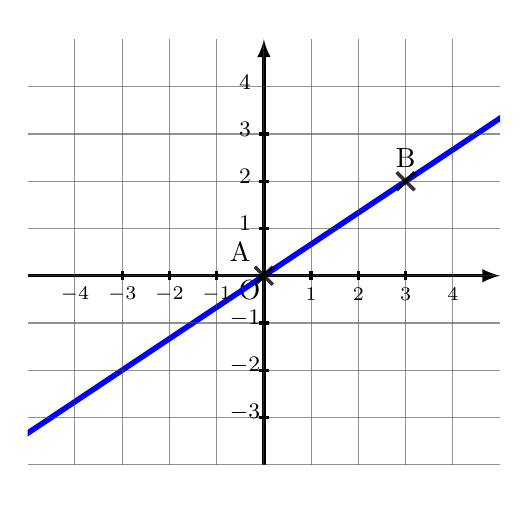
\begin{tikzpicture}[baseline,scale = 0.6]

    \tikzset{
      point/.style={
        thick,
        draw,
        cross out,
        inner sep=0pt,
        minimum width=5pt,
        minimum height=5pt,
      },
    }
    \clip (-5,-4.25) rectangle (5,5.25);
    	\draw [color={black}] (-0.3,-0.3) node[anchor = center,scale=1, rotate = 0] {O};
	\draw[color={blue},line width = 2] (-41.55,-27.7)--(44.55,29.7);
	\draw[color ={black},line width = 1.2,>=latex,->] (-5,0)--(5,0);
	\draw[color ={black},line width = 1.2,>=latex,->] (0,-4)--(0,5);
	\draw[color ={black},opacity = 0.4] (-5,1)--(5,1);
	\draw[color ={black},opacity = 0.4] (-5,-1)--(5,-1);
	\draw[color ={black},opacity = 0.4] (-5,2)--(5,2);
	\draw[color ={black},opacity = 0.4] (-5,-2)--(5,-2);
	\draw[color ={black},opacity = 0.4] (-5,3)--(5,3);
	\draw[color ={black},opacity = 0.4] (-5,-3)--(5,-3);
	\draw[color ={black},opacity = 0.4] (-5,4)--(5,4);
	\draw[color ={black},opacity = 0.4] (-5,-4)--(5,-4);
	\draw[color ={black},opacity = 0.4] (1,-4)--(1,5);
	\draw[color ={black},opacity = 0.4] (-1,-4)--(-1,5);
	\draw[color ={black},opacity = 0.4] (2,-4)--(2,5);
	\draw[color ={black},opacity = 0.4] (-2,-4)--(-2,5);
	\draw[color ={black},opacity = 0.4] (3,-4)--(3,5);
	\draw[color ={black},opacity = 0.4] (-3,-4)--(-3,5);
	\draw[color ={black},opacity = 0.4] (4,-4)--(4,5);
	\draw[color ={black},opacity = 0.4] (-4,-4)--(-4,5);
	\draw[color ={gray},opacity = 0.3] (-5,0)--(5,0);
	\draw[color ={gray},opacity = 0.3] (-5,1)--(5,1);
	\draw[color ={gray},opacity = 0.3] (-5,-1)--(5,-1);
	\draw[color ={gray},opacity = 0.3] (-5,2)--(5,2);
	\draw[color ={gray},opacity = 0.3] (-5,-2)--(5,-2);
	\draw[color ={gray},opacity = 0.3] (-5,3)--(5,3);
	\draw[color ={gray},opacity = 0.3] (-5,-3)--(5,-3);
	\draw[color ={gray},opacity = 0.3] (-5,4)--(5,4);
	\draw[color ={gray},opacity = 0.3] (-5,-4)--(5,-4);
	\draw[color ={gray},opacity = 0.3] (0,-4)--(0,5);
	\draw[color ={gray},opacity = 0.3] (1,-4)--(1,5);
	\draw[color ={gray},opacity = 0.3] (-1,-4)--(-1,5);
	\draw[color ={gray},opacity = 0.3] (2,-4)--(2,5);
	\draw[color ={gray},opacity = 0.3] (-2,-4)--(-2,5);
	\draw[color ={gray},opacity = 0.3] (3,-4)--(3,5);
	\draw[color ={gray},opacity = 0.3] (-3,-4)--(-3,5);
	\draw[color ={gray},opacity = 0.3] (4,-4)--(4,5);
	\draw[color ={gray},opacity = 0.3] (-4,-4)--(-4,5);
	\draw[color ={black},line width = 1.2] (0,-0.1)--(0,0.1);
	\draw[color ={black},line width = 1.2] (1,-0.1)--(1,0.1);
	\draw[color ={black},line width = 1.2] (-1,-0.1)--(-1,0.1);
	\draw[color ={black},line width = 1.2] (2,-0.1)--(2,0.1);
	\draw[color ={black},line width = 1.2] (-2,-0.1)--(-2,0.1);
	\draw[color ={black},line width = 1.2] (3,-0.1)--(3,0.1);
	\draw[color ={black},line width = 1.2] (-3,-0.1)--(-3,0.1);
	\draw[color ={black},line width = 1.2] (-0.1,0)--(0.1,0);
	\draw[color ={black},line width = 1.2] (-0.1,1)--(0.1,1);
	\draw[color ={black},line width = 1.2] (-0.1,-1)--(0.1,-1);
	\draw[color ={black},line width = 1.2] (-0.1,2)--(0.1,2);
	\draw[color ={black},line width = 1.2] (-0.1,-2)--(0.1,-2);
	\draw[color ={black},line width = 1.2] (-0.1,3)--(0.1,3);
	\draw[color ={black},line width = 1.2] (-0.1,-3)--(0.1,-3);
	\draw (1,-0.4) node[anchor = center, rotate=0] {\scriptsize \color{black}{$1$}};
	\draw (2,-0.4) node[anchor = center, rotate=0] {\scriptsize \color{black}{$2$}};
	\draw (3,-0.4) node[anchor = center, rotate=0] {\scriptsize \color{black}{$3$}};
	\draw (4,-0.4) node[anchor = center, rotate=0] {\scriptsize \color{black}{$4$}};
	\draw (-1,-0.4) node[anchor = center, rotate=0] {\scriptsize \color{black}{$-1$}};
	\draw (-2,-0.4) node[anchor = center, rotate=0] {\scriptsize \color{black}{$-2$}};
	\draw (-3,-0.4) node[anchor = center, rotate=0] {\scriptsize \color{black}{$-3$}};
	\draw (-4,-0.4) node[anchor = center, rotate=0] {\scriptsize \color{black}{$-4$}};
	\draw (-0.4,1.1) node[anchor = center, rotate=0] {\footnotesize \color{black}{$1$}};
	\draw (-0.4,2.1) node[anchor = center, rotate=0] {\footnotesize \color{black}{$2$}};
	\draw (-0.4,3.1) node[anchor = center, rotate=0] {\footnotesize \color{black}{$3$}};
	\draw (-0.4,4.1) node[anchor = center, rotate=0] {\footnotesize \color{black}{$4$}};
	\draw (-0.4,-0.9) node[anchor = center, rotate=0] {\footnotesize \color{black}{$-1$}};
	\draw (-0.4,-1.9) node[anchor = center, rotate=0] {\footnotesize \color{black}{$-2$}};
	\draw (-0.4,-2.9) node[anchor = center, rotate=0] {\footnotesize \color{black}{$-3$}};
	\draw[color ={black},line width = 1.25,opacity = 0.8] (2.81,2.19)--(3.19,1.81);\draw[color ={black},line width = 1.25,opacity = 0.8] (2.81,1.81)--(3.19,2.19);
	\draw[color ={black},line width = 1.25,opacity = 0.8] (-0.19,0.19)--(0.19,-0.19);\draw[color ={black},line width = 1.25,opacity = 0.8] (-0.19,-0.19)--(0.19,0.19);
	\draw [color={black}] (-0.5,0.5) node[anchor = center,scale=1, rotate = 0] {A};
	\draw [color={black}] (3,2.5) node[anchor = center,scale=1, rotate = 0] {B};

\end{tikzpicture}\\
	\item Soit la suite $(u_n)$ définie  par $u_0 = 4$ et pour $n \in \mathbb{N}$, 
    $u_{n+1} = -3u_n +2$.\\
    $u_2=$ $\ldots$
	%\item $P(A\cap B)=0{,}15$\\$P(A)=0{,}3\,\,;\,\,P(B)=0{,}5$\\$A$ et $B$ sont indépendants.\\\\	$\square\;$ Vrai\qquad $\square\;$ Faux\qquad 
	\item Le discriminant du trinôme $x^2-3x-2$ est  $\ldots$
	\item Un sportif court $3\,500$ m  en $15$ min.\\
      Quelle est sa vitesse en km/h ?
	\item $f(x)=\dfrac{1}{2}x^2+3x-7$\\
    $f'(x)=$ $\ldots$
	
	%\item $q\neq 1$ \\$q+q^2+\ldots+q^{12}=$ \\	$\square\;$ $\dfrac{q-q^{13}}{1-q}$ \qquad $\square\;$ $\dfrac{1-q^{13}}{1-q}$\qquad 
	%\item $f(x)=-2x^2+7$\\
    %$f'(1)=$ $\ldots$
	%\item Solutions de $(x-2)(x-4)  > 0$\\
	%\item Soit $f\,:\,x\longmapsto x(x-8) $\\
    %La représentation graphique $\mathcal{C}_f$ a pour axe de symétrie la droite d’équation :\\	$\square\;$ $x=8$\qquad $\square\;$ $x=4$\qquad $\square\;$ $x=-4$\qquad 
	\item Le double  de $2^{34}=2^?$\\$?=\ldots$
	\item Augmenter une quantité de $300$ \% revient à la multiplier par : $\ldots$
	\item $1,25$ h $=$ $\ldots$ h $\ldots$ min
	\item Compléter\\ 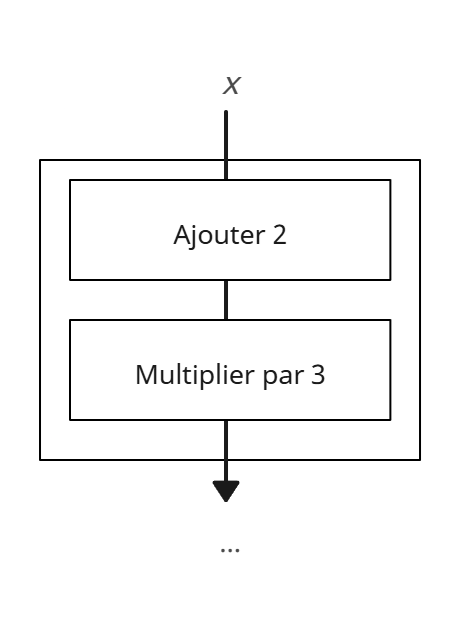
\includegraphics[width=5cm]{Can3.png}
	\item Je lance $n$ fois un dé équilibré.\\
    Quelle est la probabilité de n'obtenir que des 6 ?
\end{enumerate}
\vfill\null
\columnbreak
Mon temps : $\ldots$\\[.5em]
Mon score : $\ldots$/20
\end{multicols}
\newpage

\begin{multicols}{2}
    \classe{\terminale Comp}
\titre{
\includegraphics[width=3cm]{CAN.png} Corrigé 3}
\maketitle

\begin{enumerate}[itemsep=1em]
    \item On peut calculer ainsi : \\
        $\begin{aligned}
        0{,}5\times7&=0,1\times 5\times7\\
        &=0,1\times 35\\
        &={\color[HTML]{f15929}\boldsymbol{3{,}5}}
        \end{aligned}$
    \item Le point $A$ est sur la parabole si son ordonnée est égale à l'image de son abscisse. \\
        $\begin{aligned}
            f(1)&=1^2-1\\
            &=0
            \end{aligned}$
            \\
            Le point $A$ est bien sur la parabole.\\ L'affirmation est {\bfseries \color[HTML]{f15929}VraiE}
    \item $\begin{aligned}
          (x+1)(x-1)&=x^2-x+x-1\\
          &={\color[HTML]{f15929}\boldsymbol{x^2-1}}
          \end{aligned}$\\Le terme en $x^2$ vient de $x\times 1x=x^2$.\\Le terme en $x$ vient de la somme de $x \times (-1)$ et de $1 \times 1x$.\\Le terme constant vient de $1\times (-1)= -1$.
    \item $\begin{aligned}
          4+\dfrac{1}{3} &= \dfrac{4 \times 3}{3} + \dfrac{1}{3} \\
          &= \dfrac{12}{3} + \dfrac{1}{3}\\
          &  ={\color[HTML]{f15929}\boldsymbol{\dfrac{13}{3}}}
          \end{aligned}$
\vfill\null
\columnbreak
    \item $30\,\%$ de $70 = {\color[HTML]{f15929}\boldsymbol{21}}$\\ Prendre $30\,\%$  de $70$ revient à prendre $3\times 10\,\%$  de $70$.\\
          Comme $10\,\%$  de $70$ vaut $7$ (pour prendre $10\,\%$  d'une quantité, on la divise par $10$), alors
          $30\,\%$ de $70=3\times 7=21$.
         
    \item $\dfrac{11}{4}={\color[HTML]{f15929}\boldsymbol{2{,}75}}$
    \item Comme $0{,}74-1=-0{,}26$, multiplier par $0{,}74$ revient à diminuer de ${\color[HTML]{f15929}\boldsymbol{26}}\,\%$. 
    \item La raison de la suite est donnée par le quotient $\dfrac{u_1}{u_0}=\dfrac{-48}{8}={\color[HTML]{f15929}\boldsymbol{-6}}$.
    \item Comme $81 < 83 < 100$, alors 
        ${\color[HTML]{f15929}\boldsymbol{9}} < \sqrt{83} < {\color[HTML]{f15929}\boldsymbol{10}}$.
    \item On procède par étapes successives :\\
          On commence par isoler $7x$ dans le membre de gauche en retranchant
          $3$ dans chacun des membres, puis on divise
          par $7$ pour obtenir la solution : \\
           $\begin{aligned}
           7x+3&=2\\
          7x&=2-3\\
          7x&=-1\\
          x&=\dfrac{-1}{7}    
          \end{aligned}$\\
          La solution de l'équation est : ${\color[HTML]{f15929}\boldsymbol{\dfrac{-1}{7}}}$.
          
    %\item $\begin{aligned}
    %      \dfrac{17\pi}{7}&=\dfrac{14\pi}{7}+\dfrac{3\pi}{7}\\
    %      &=2\pi+{\color[HTML]{f15929}\boldsymbol{\dfrac{3\pi}{7}}}
    %      \end{aligned}$
\vfill\null
\columnbreak
    %\item $(2x-3)$ est un facteur commun.\\
    %      $\begin{aligned}
    %      -2(2x-3)+(2x-3)^2
    %      &=(2x-3)(-2+(2x-3))\\
    %      &={\color[HTML]{f15929}\boldsymbol{(2x-3)(2x-5)}}\end{aligned}$
    
    \item En utilisant les deux points $A$ et $B$, on détermine le coefficient directeur $m$ de la droite : \\
        $m=\dfrac{y_B-y_A}{x_B-x_A}=\dfrac{2}{3}$.\\
             L' ordonnée à l'origine est $0$, ainsi l'équation réduite de la droite est ${\color[HTML]{f15929}\boldsymbol{y=\dfrac{2}{3}x}}$.
    
    \item On calcule d'abord $u_1$ : \\   
          $\begin{aligned}
          u_1&=-3\times u_0 +2\\
          u_1&=-3\times 4 +2\\
          &=-10     
          \end{aligned}$\\
          On obtient donc pour $u_2$ :\\
          $\begin{aligned}
          u_2&=-3\times u_1 +2\\
          u_2&=-3\times (-10) +2\\
          &={\color[HTML]{f15929}\boldsymbol{32}}     
          \end{aligned}$
    %\item $A$ et $B$ sont indépendants si $P(A\cap B)=P(A)\times P(B)$.\\
    %    Comme :\\$\begin{aligned}
    %    P(A)\times P(B)&=0{,}3\times 0{,}5\\
    %    &=0{,}15
    %    \end{aligned}$\\On obtient l'égalité  $P(A\cap B)=P(A)\times P(B)$.\\
    %    Les événements $A$ et $B$ sont donc indépendants.\\ L'affirmation est {\bfseries \color[HTML]{f15929}VraiE}.
%\vfill\null
%\columnbreak
    \item  $\Delta=b^2-4ac$ avec $a=1$, $b=-3$ et $c=-2$.\\
          $\begin{aligned}
          \Delta&=(-3)^2-4\times 1\times (-2) \\
          &={\color[HTML]{f15929}\boldsymbol{17}} 
          \end{aligned}$
    \item En $1$ heure, il parcourt $4$ fois plus de distance  qu'en $15$ minutes, soit $4\times 3\,500=
          14\,000$ m.\\
          Sa vitesse est donc ${\color[HTML]{f15929}\boldsymbol{14}}$ km/h.
    \item  On détermine la fonction dérivée :\\
          $\begin{aligned}
          f'(x)&=\dfrac{1}{2}\times 2x -7\\
          &={\color[HTML]{f15929}\boldsymbol{x+3}}     
          \end{aligned}$
      
    %\item $(x-2)(x-4)$ est l'expression factorisée d'une fonction polynôme du second degré de la forme $a(x-x_1)(x-x_2)$.\\
    %    Les racines sont $x_1=2$ et $x_2=4$. \\
    %    Le polynôme est du signe de $a=1$ (donc positif) sauf entre ses racines.\\
    %    L'ensemble solution est donc :  ${\color[HTML]{f15929}\boldsymbol{]-\infty;2[\cup]4;+\infty[}}$.   
         
    %\item Les racines de ce polynôme du second degré sont $x_1=8$ et $x_2=0$.\\
    %    L'axe de symétrie est donné par la moyenne des racines : $x=\dfrac{x_1+x_2}{2}$, soit $x=\dfrac{8+0}{2}$, c'est-à-dire ${\color[HTML]{f15929}\boldsymbol{x=4}}$.
    \item Le double de $2^{30}$ est $2\times 2^{34}=2^{{\color[HTML]{f15929}\boldsymbol{35}}}$.
    \vfill\null
    \columnbreak
    \item Augmenter une quantité de $300\,\%$ revient à la multiplier par $1+\dfrac{300}{100}={\color[HTML]{f15929}\boldsymbol{4}}$.

    \item $1,25$ h $=1$ h $0,25\times 60$ min $=${\color[HTML]{f15929}{$1$ h $15$ min}}.
    \item Ce programme de calcul donne {\color[HTML]{f15929}{$3(x+2)$}} $=3x+6$.
    \item On répète $n$ fois un événement qui a une probabilité de $\dfrac{1}{6}$ de se produire.\\
          La probabilité de n'obtenir que des 6 est {\color[HTML]{f15929}{$\left(\dfrac{1}{6}\right)^n$}} $=\dfrac{1}{6^n}$.
       
\end{enumerate}
\end{multicols}
\end{document}